%~~~~~~~~~~~~~~~~~~~~~~~~~~~~~~~~~~~~~~~~~~~~~~~~~~~~~~~~~~~~~~~~~~~~~~~~
% $Id: ProfileCycleModel.tex,v 1.2 2008/07/14 17:02:19 swift Exp $
%~~~~~~~~~~~~~~~~~~~~~~~~~~~~~~~~~~~~~~~~~~~~~~~~~~~~~~~~~~~~~~~~~~~~~~~~
% RCS Log:
%
% $Log: ProfileCycleModel.tex,v $
% Revision 1.2  2008/07/14 17:02:19  swift
% Added compensator hyper-retraction feature to allow floats to be
% parked at mid-water pressures.
%
% Revision 1.1  2006/11/03 19:08:57  swift
% Added user manual to CVS control.
%
% Revision 1.3  2006/07/10 22:24:49  swift
% Modifications to bring the manual up to date with
% changes to the SeaBird CTD firmware (v1.1c).
%
% Revision 1.2  2006/04/10 16:11:51  swift
% Added the subsection describing the deep-profile cycle.
%
% Revision 1.1  2005/12/27 23:29:06  swift
% Initial revision
%
%~~~~~~~~~~~~~~~~~~~~~~~~~~~~~~~~~~~~~~~~~~~~~~~~~~~~~~~~~~~~~~~~~~~~~~~~

\newcommand{\Pn}{P$_{N_2}$}

\section{Controlling \iridium\ \apex\ behavior: A parametric model.}
\label{sec:ProfileCycleModel}

The \iridium\ \apex\ firmware is highly configurable so that the user can
control float behavior by adjusting the values of more than 20 parameters
and by selecting several optional modes and features.  

\subsection{Sample missions.}
\label{sec:SampleMissions}

The ability to configure the float within a 20(plus) dimensional parameter
space means that that range of possible float behaviors is practically
infinite.  However, some general characteristics span the whole parameter
space while many potentially useful kinds of missions are excluded
entirely.  Figures~\ref{fig:P4P}, \ref{fig:P1P}, and \ref{fig:P254P}
represent common mission cycles within the usable parameter space.

Figure~\ref{fig:P4P} represents the most general kind of mission cycle and
is referred to as \emph{Park-n-Profile} (PnP).  The original motivation for
PnP was as a mechanism to balance the competing objectives of energy savings
versus direct measurement of salinity drift in the deeper water.  The basic
idea was to collect most profiles from the park level but occasionally
execute a deep profile to facilitate evaluation of CTD performance.  The
``$n$'' in PnP refers to the cycle length of the PnP mechanism; every $n^{th}$
profile is a deep profile.  

\begin{figure}[htbp]
  \begin{center}
    \leavevmode
    \mbox{\includegraphics[scale=0.5,clip,draft=false]{P4P.ps}}
    \caption{Schematic of a PnP mission with cycle length $n=4$.  The park
      level is the same for all profiles.  Every fourth profile is a deep
      profile.  The shallow blip prior to the (special) first profile
      represents pressure activation.}
    \label{fig:P4P}
  \end{center}
\end{figure}

The first profile is special because it is executed immediately after the
mission prelude, does not drift at the park level, and is also a deep
profile.  The first profile will be telemetered within 24~hours after the
mission is activated.  The exact timing will depend on the user's specific
parameter selections.  This feature was implemented to satisfy the
often-heard request for a profile to be executed immediately after
deployment.

Figure~\ref{fig:P1P} represents a PnP mission with $n=1$ (ie., a P1P mission).
In this way, PnP firmware can be programmed to collect lagrangian data from
a shallower level while still being able to collect deep profiles.  As with
the P4P mission in Figure~\ref{fig:P4P}, the first profile is executed
immediately after the mission prelude.

\begin{figure}[htbp]
  \begin{center}
    \leavevmode
    \mbox{\includegraphics[scale=0.5,clip,draft=false]{P1P.ps}}
    \caption{Schematic of a PnP mission with cycle length $n=1$.  Every
      profile parks shallow but profiles deep.  The shallow blip prior to
      the (special) first profile represents pressure activation.}
    \label{fig:P1P}
  \end{center}
\end{figure}

Figure~\ref{fig:P254P} represents a degenerate case of the PnP model where
$n$ is large and the park level has been chosen to be deep.  This mission
cycle is so common amongst \apex\ users that it was implemented as a special
case.  The value $n=254$ is a special sentinel value that disables the PnP
feature so that only park-level mission parameters (ie., park pressure and
park piston position) are used for controlling the profile cycle; the
profile-level parameters (ie., profile pressure and profile piston position)
are ignored.

\begin{figure}[htbp]
  \begin{center}
    \leavevmode
    \mbox{\includegraphics[scale=0.5,clip,draft=false]{P254P.ps}}
    \caption{Schematic of a degenerate PnP mission with cycle length n=254.
      Every cycle parks and profiles from the park level.  The shallow blip
      prior to the (special) first profile represents pressure activation.}
    \label{fig:P254P} 
  \end{center}
\end{figure}

As with the previous two examples, the first profile is executed
immediately after the mission prelude.

\subsection{Deconstructing the profile cycle.}
\label{sec:DeconstructProfileCycle}

Details of the firmware architecture and design are outside the scope of
this user manual.  However, deconstructing the profile cycle into its
constituent elements will give meaning to many of the configuration
parameters.

The \apf\ firmware design makes fundamental use of the concept of ``sequence
points'' for controlling the flow of the profile cycle.  A sequence point is
defined to be a point where one phase of the mission cycle transitions to
the next phase.  Most of the sequence points are based on time but there are
several sequence points that are event-based.  Given a properly functioning
\apf\ controller, the firmware guarantees the phase transition at each
sequence point regardless of the health of any other float component.

The schematics below illustrate different parts of the mission cycle:
\begin{enumerate}
\item The pressure-activation phase.
\item The mission prelude.
\item A profile from the park level.
\item A deep profile.
\end{enumerate}

\subsubsection{Pressure-activation phase (\emph{optional}).}

The pressure-activation feature is an optional phase of the mission that
preceeds the mission prelude.  It was designed to accomodate requests from
ship's crew to be able to deploy the float without being required to start
it with a magnet.  One event-based sequence point is implemented that
activates the mission prelude if the pressure exceeds the activation
threshold (ie., 25~decibars).

\begin{minipage}{6in}
   \begin{verbatim}
                            |----------------- L ----------------------|
    -+----------------+-----+-------+----------------------------------+- Time
    P|                 .    |      .                                    .    
    r|                   .  |     .       Sequence Points                 .   
    e|                      .    .        -----------------------           .  
    s|                      B   .         L = Mission prelude                  .
    s|                                    B = Pressure-activation
    u|
    r|
    e|
  \end{verbatim}
\end{minipage}

Pressure activation mode is not ``on'' by default.  The user must enable
pressure activation mode via the interactive user interface (see
Section~\ref{sec:MissionConfiguration}).  Enabling the pressure activation
mode immediately induces the firmware to perform a self-test of the float.
 
In order for pressure activation to work the float has to be able to sink
from the surface down to the activation pressure (ie., 25~decibars).
Obviously, if the float is too buoyant to sink then it can never
self-activate.  Enabling pressure activation mode causes the firmware to put
the float into a state of minimum buoyancy; the buoyancy pump is fully
retracted to deflate the oil bladder and the air solenoid valve is opened to
deflate the air bladder.  Then the firmware enters a nonterminating loop
where the the CTD is queried for pressure every two hours.  If the pressure is
less than the activation pressure then the \apf\ controller puts itself back
to sleep for another two hours.  However, if the pressure exceeds the
activation threshold then the firmware launches the mission and enters the
mission prelude.

\subsubsection{The mission prelude.}

The purpose of the mission prelude is mainly to allow the float to transmit
a fix of its deployment location and to telemeter its mission programming
parameters.  The mission prelude is the time period between mission
activation and the first descent.  The sequence point 'L' is time-based and
is the transition between the mission prelude and the first descent.  The
period of the mission prelude is user-defined (see
Section~\ref{sec:MissionConfiguration}).
   
\begin{minipage}{6in}
  \begin{verbatim}
     |--------------------------- L -----------------------------------|
    -+-----------------------------------------------------------------+- Time
    P|                                                                  .    
    r|                                              Sequence Points      .   
    e|                                              -------------------   .  
    s|                                              L = Mission prelude     .
    s|                                                                       
    u|
    r|
    e|
  \end{verbatim}
\end{minipage}

When the mission is launched either manually or else by the pressure
activation mechanism, the firmware puts the float into a state of maximum
buoyancy by fully extending the buoyancy pump to inflate the oil bladder and
then inflating the air bladder.

\subsubsection{Profile from park depth.}
\label{sec:ParkProfileCycle}

The profile cycle for a shallow profile consists of four phases (each
associated with a time-based sequence point): descent (F), park (K), profile
(P), and telemetry (C).  Two additional event-based sequence points (S,T)
ordinarily cause phase transition before their associated time-outs force
the phase transition.

\begin{minipage}{6in}
\begin{verbatim}
     |--------------------------------------------------- C ----------------|     
     |------------------------------ P ---------------|                     |     
     |----------------- K -------------|              |                     |     
     |--- F -----|                     |           S  |                T    |     
    -+-----------+---------------------+-----------+-------------------+----+- Time
    P|.          |                     |         .                      .    
    r| .         |                     |       .       Sequence Points   .   
    e|  .        |                     |     .         ---------------    .  
    s|    .      |                     |   .           F = Descent          .
    s|       .   |                     | .             K = Park
    u|           . . . . . . . . . . . .               S = Surface detect
    r|                                                 P = Profile           
    e|                                                 T = Telemetry
     |                                                 C = Cycle
\end{verbatim}                    
\end{minipage}

This is the simplest kind of profile cycle which \apex\ floats have executed
since their initial development.  The float sinks to its park depth, drifts
for a period of time, profiles to the surface, and then telemeters its data.
However, unlike \apex\ with ARGOS telemetry, the length of time for each
profile cycle is not fixed.  The profile cycle for \iridium\ \apex\ ends as
soon as the telemetry is successfully completed or the profile cycle
time-out (C) expires, whichever happens first.  Typically, an \iridium\
float is on the surface for only 15 minutes or so before the next profile
cycle begins.

For this kind of profile cycle, the end of the park phase (K) coincides with
the end of the ``down-time'' and the beginning of the ``up-time''.  The
sequence point C coincides with the end of the up-time.  The (maximum)
length of the profile cycle is the down-time plus the up-time. 

\begin{description}

\item[Descent phase\label{DescentPhase}]---The profile cycle starts with
  the descent phase.  The float queries the CTD for the surface pressure and
  then the buoyancy pump is retracted to the park position.  The float sinks
  until the descent period expires (ie., the firmware forces a phase
  transition at the sequence-point~F in the schematic above).  Hourly
  pressure measurements are logged as well as one at the completion of the
  buoyancy pump retraction.  These pressure measurements are referred to as
  \emph{descent marks} and are telemetered as engineering data.
  
  \textbf{Special notes for floats with \NComp:\label{DescentPhaseNComp}}
  The gas pressure (\Pn) in the \NComp\ plays an important role during the
  descent phase.  While the float is at the surface, the \NComp\ piston is
  fully extended which adds $\sim$80~grams of buoyancy to the float.  In
  order to descend back down to the park level, the buoyancy pump must
  reduce the buoyancy enough to descend deeper than the gas pressure \Pn.
  To accomplish this, the piston is retracted beyond the park piston
  position.  This is referred to as \emph{compensator hyper-retraction}.
  Near the end of the descent phase, the piston is extended back to the park
  position.  This allows floats with \NComp\ to park at any depth greater
  than 850~dbars.  \textbf{Warning:} The \NComp\ renders the float buoyantly
  unstable in the range of pressures $\sim$400--700~decibars.  Therefore,
  such floats must be parked outside this range.

\item[Park phase\label{ParkPhase}]---Active ballasting is accomplished and
  park-level PT measurements are collected during the park phase.  The \apf\
  wakes once each hour to accomplish these tasks.  A PTS sample is collected
  at the end of the park phase.
  
  \begin{description}
  \item[Active ballasting:] The float wakes each hour to monitor the
    pressure and make buoyancy adjustments if three \textbf{consecutive}
    measurements violate a 10~decibar dead-band on either side of the
    user-specified park pressure.  Measurements that are within the
    dead-band or that completely cross the dead-band reset the violation
    counter and will not induce buoyancy adjustments.
    
  \item[Park-level PT samples:] The float collects hourly low-power PT
    measurements and telemeters them as hydrographic data.  Refer to
    Section~\ref{sec:PtSample} for their data format.  Hourly salinity data
    are not measured due to energy considerations.
    
  \item[Park-level PTS sample:] The float collects one PTS sample at the end
    of the park phase (K).  Refer to Section~\ref{sec:LowResPtsSample} for
    its data format.
  \end{description}
  
\item[Profile phase\label{ProfilePhase}]---As might be expected, the profile
  phase is the most complicated of the profile cycle.  Three asynchronous
  processes are active during the profile cycle: Ascent rate control,
  hydrographic sampling, and surface detection.  These processes operate on
  a 10~second heartbeat; the \apf\ controller sleeps for 10~seconds then
  wakes to attend to these processes before going back to sleep.

  \begin{description}
  \item[Ascent rate control:] As an initialization step of the profile
    phase, the buoyancy engine adds a user-specified initial increment of
    buoyancy to start the float ascending toward the surface.  Thereafter,
    the firmware monitors the pressure at 5~minute intervals to determine if
    the average ascent rate has been maintained above 0.08~decibars/sec.  If
    the ascent rate falls below this threshold then the buoyancy engine adds
    a user-specified increment of buoyancy.
    
  \item[Hydrographic sampling:] \iridium\ \apex\ is designed to collect
    hydrographic profiles with relatively high vertical resolution.  The
    \sbe\ \ctd\ has a continuous profiling (CP) mode that runs
    asynchronously and autonomously from the float's \apf\ controller.  When
    CP-mode is active, the \ctd\ collects 1-Hz samples and stores them
    internally in nonvolatile memory.  
    
    The \apf\ shuts down CP-mode 4~decibars below the surface to avoid
    contaminating the conductivity cell with ingested surface scum.  To
    protect against pressure-sensor drift, the \apf\ commands the \sbe\ to
    shut down 4~decibars deeper than the most recent surface pressure
    measurement.  As a fail-safe measure, the \sbe\ will shut itself down
    when its pressure sensor reaches 2~decibars (but no attempt is made to
    account for drift of the pressure sensor).
    
    After the float reaches the surface the \apf\ commands the \sbe\ to sort
    the 1-Hz samples into 2~decibar bins and compute the arithmetic mean of
    the samples in each bin.  The resulting bin-averaged profiles have
    2~decibar resolution though we often refer to them as ``high
    resolution'' or ``continuous profiles''.  These high resolution profiles
    are telemetered using the format defined in
    Section~\ref{sec:HiResPtsSample}.
    
    The \sbe\ also has a spot-sampled mode that is roughly simlar to the
    Sbe41 used on ARGOS \apex\ floats.  This \iridium\ firmware implements an
    optional mixed-mode sampling strategy in order to save energy in the
    deep water where gradients are small.  At the user's discretion, the
    float can be programmed to collect spot samples in the deep water and
    automatically transistion to continuous profiling when the float ascends
    to the \emph{CP Activation Pressure}.  To disable this feature and force
    continuous profiling from top to bottom then the user should specify the
    activation pressure to be deeper than the float's operating range.
    Spot-samples are formated according to Section~\ref{sec:LowResPtsSample}
    and collected according to a pressure table that is hard-coded in
    firmware.
    
  \item[Surface detection:] The surface detection algorithm terminates true
    when the float ascends to a pressure that is within 4~decibars of the
    most recent surface pressure measurement\footnote{Actually, the surface
      detection algorithm is more complicated than this but the
      complications handle pathological situations.  Refer to the C source
      code (src/profile.c) in your distribution.}.  Surface detection causes
    the profile to be terminated, another increment of buoyancy to be
    added by the buoyancy pump, and transition to the telemetry phase.
  \end{description}

\item[Telemetry phase\label{TelemetryPhase}]---If the end of the antenna is
  even a centimeter below the water's surface then telemetry will not be
  possible.  Therefore, the telemetry phase starts with precise surface
  detection using its SkySearch algorithm.  The heart of this algorithm
  involves attempting to register the LBT with the \iridium\ system.  If the
  algorithm terminates true then GPS acquisition and telemetry can proceed;
  otherwise, the buoyancy engine adds another increment of buoyancy and
  sleeps for one telemetry-retry period before repeating the attempt.

  After determining that the float can see the sky then the LBT is shut down
  and the GPS engine is used to acquire the float's location.  After
  acquiring the fix then the GPS is shut down and the LBT is reregistered
  with the \iridium\ system.  The float places a call via the \iridium\
  system to the remote host and logs in using the float's username and
  password.  Once logged into the remote host, the float downloads its new
  configuration from the remote host and uploads its hydrographic and
  engineering data to the remote host.  Finally, the float logs out of the
  remote host and reprograms its mission paramters according to the new
  configuration file that it just received from the remote host.
\end{description}

\subsubsection{Deep profile.}
\label{sec:DeepProfileCycle}

For PnP cycle lengths less than 254, the first profile cycle will be a deep
one as will profile cycles for which the internal profile counter (PrfId) is
an integral multiple of the profile cycle length.  For example, a P4P
mission will execute a deep profile cycle when the internal profile counter
is 1, 4, 8, 12, and so on.  The following C source code represents the test
executed by firmware to determine if the current profile cycle is a deep
one:

   \begin{verbatim}
   (PnpCycleLength<254 && ((!(PrfId%PnpCycleLength)) || PrfId==1) ? Yes : No;
   \end{verbatim}                    

The profile cycle for a deep profile consists of five phases (each
associated with a time-based sequence point): descent (F), park (K),
deep-descent (D), profile (P), and cycle (C).  Three additional event-based
sequence points (Q,S,T) ordinarily cause phase transition before their
associated time-outs force the phase transition.
   
\begin{minipage}{6in}
   \begin{verbatim}
     |------------------------------------------------------ C -------------|     
     |--------------------------------- P ------------|                     |     
     |----------------- D --------|                   |                     |     
     |------- K -------------|    |                   |                     |     
     |--- F -----|           |    |                S  |                T    |     
    -+-----------+-----------+----+----------------+-------------------+------- Time
    P|.          |           |    |              .                      .    
    r| .         |           |    |            .       Sequence Points   .   
    e|  .        |           |    |          .         ---------------    .  
    s|    .      |           |    |        .           F = Descent          .
    s|       .   |           |    |      .             K = Park                        
    u|           . . . . . . .    |    .               Q = DeepProfile 
    r|                            |  .                 D = DeepDescent
    e|                        .   |.                   S = SurfaceDetect
     |                           .                     P = Profile
     |                         .                       T = Telemetry 
     |                         Q                       C = Cycle                             
   \end{verbatim}
\end{minipage}

For this kind of profile cycle, the end of the deep-descent phase (D)
coincides with the end of the ``down-time'' and the beginning of the
``up-time''.  The sequence point C coincides with the end of the up-time.
The (maximum) length of the profile cycle is the down-time plus the up-time.

\begin{description}

\item[Descent phase]---Refer to description on page~\pageref{DescentPhase}.

\item[Park phase]---Refer to description on page~\pageref{ParkPhase}.  The
  park phase is shortened for the deep profile cycle in order to allow time
  to descend from the park level to the deep target pressure.

\item[Deep descent phase]---The purpose of the deep descent phase is to
  allow the float to descend from the park level (eg., 1000~dbars) to the
  pressure where the deep profile should begin (eg., 2000~dbars).  The
  maximum time allowed for the deep descent phase is user specified (see
  Section~\ref{sec:MissionConfiguration}).

  The deep descent phase begins by retracting the piston from the park
  piston position to the profile piston position.  During the descent, the
  pressure is monitored every five minutes to determine of the target
  pressure has been reached (ie., sequence point Q).

  \begin{description}

  \item[Sequence point Q]---If the float descends to its deep target
    pressure before the deep descent phase times out then the profile piston
    position is incremented by one count (but no piston extension occurs).
    The intent is to reduce the descent speed during the next deep profile
    so that the float will reach the target pressure closer to the end of
    the down time (ie., sequence point D).

  \item[Sequence point D]---If the deep descent period times out before the
    target pressure is reached then the profile piston position is
    decremented by one count (but no piston retraction occurs).  The intent
    is to increase the descent speed during the next deep profile so that
    the float will reach the target pressure before the end of the down time
    (ie., sequence point D).

  \end{description}

  Transition to the profile phase is forced at either sequence point Q or D.

\item[Profile phase]---Refer to description on page~\pageref{ProfilePhase}.

\item[Telemetry phase]---Refer to description on page~\pageref{TelemetryPhase}.


\end{description}


%%% Local Variables: 
%%% mode: latex
%%% TeX-master: "IridiumApex"
et
%%% End: 
